\chapter{ Spread of Zika virus on a small world network }

\begin{figure}[h!]
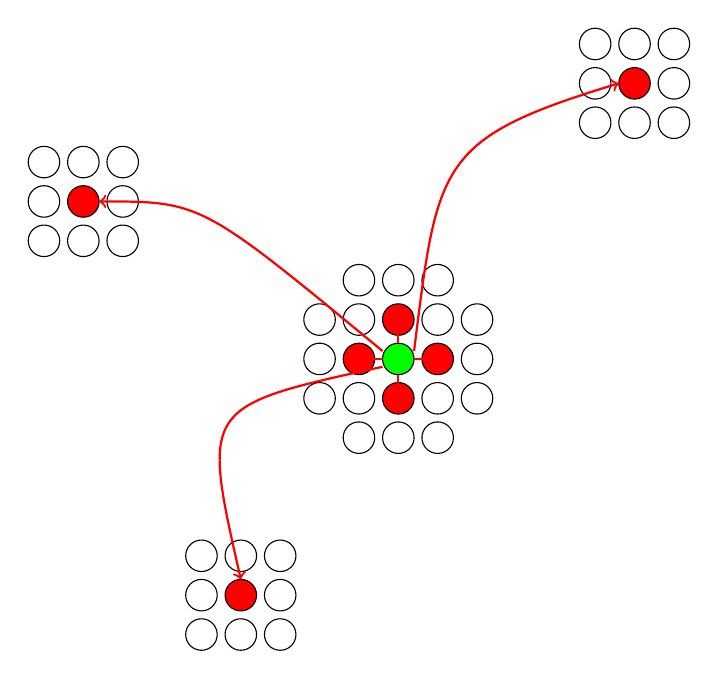
\begin{tikzpicture}
\draw (-2,5.5) circle (0.2cm);
\draw (-2,5.0) circle (0.2cm);
\draw (-2,4.5) circle (0.2cm);
\draw (-1.5,5.5) circle (0.2cm);
\filldraw[fill=red!, draw=black] (-1.5,5.0) circle (0.2cm);
\draw (-1.5,4.5) circle (0.2cm);
\draw (-1,5.5) circle (0.2cm);
\draw (-1,5.0) circle (0.2cm);
\draw (-1,4.5) circle (0.2cm);
\draw (2,2) circle (0.2cm);
\filldraw[fill=red!, draw=black](2,3) circle(0.2 cm);
\draw (2.5,2) circle (0.2cm);
\filldraw[fill =green, draw =black](2.5,3) circle(0.2 cm);
\draw (2,2.5) circle (0.2cm);
\draw(2,3.5) circle(0.2 cm);
\filldraw[fill=red!, draw=black] (2.5,2.5) circle (0.2cm);
\filldraw[fill=red!, draw=black](2.5,3.5) circle(0.2 cm);
\draw (3,2) circle (0.2cm);
\filldraw[fill=red!, draw=black](3,3) circle(0.2 cm);
\draw (3,2.5) circle (0.2cm);
\draw(3,3.5) circle(0.2 cm);
\draw(1.5,2.5) circle (0.2cm);
\draw(1.5,3) circle (0.2cm);
\draw(1.5,3.5) circle(0.2cm);
\draw(2,4) circle(0.2cm);
\draw(3.5,2.5) circle (0.2cm);
\draw (3.5,3) circle (0.2cm);
\draw(3.5,3.5) circle (0.2cm);
\draw(2.5,4) circle(0.2 cm);
\draw(3,4) circle(0.2 cm);

\draw(0,0.5) circle (0.2cm);
\draw (0,0.0) circle (0.2cm);
\draw (0,-0.5) circle (0.2cm);
\draw (0.5,0.5) circle (0.2cm);
\filldraw[fill=red!, draw=black](0.5,0) circle (0.2cm);
\draw (0.5,-0.5) circle (0.2cm);
\draw (1,0.5) circle (0.2cm);
\draw (1,0) circle (0.2cm);
\draw (1,-0.5) circle (0.2cm);


\draw (5,6) circle (0.2cm);
\draw (5,6.5) circle (0.2cm);
\draw (5,7) circle (0.2cm);
\draw (5.5,6) circle (0.2cm);
\filldraw[fill=red!, draw=black](5.5,6.5) circle (0.2cm);
\draw (5.5,7) circle (0.2cm);
\draw (6,6) circle (0.2cm);
\draw (6,6.5) circle (0.2cm);
\draw (6,7) circle (0.2cm);

\draw[red!,thick] (2,3) --(2.3,3);
\draw[red!,thick] (3,3) --(2.7,3);
\draw[red!,thick] (2.5,3.5) --(2.5,3.2);
\draw[red!, thick] (2.5,2.5) --(2.5,2.8);

\draw[draw=red!,
preaction={->,thick,draw =red!}
] (2.7,3.1) ..controls(3,5.5) and (3,5.8) ..(5.3,6.5);
\draw[ draw =red!,thick, ->] (2.3,3.1) .. controls (0,5) and (0,5) ..(-1.3,5);

\draw [draw =red , thick, ->] (2.3,2.9).. controls (0,2.4) .. (0.5,0.2);
\end{tikzpicture}
\caption{Smallworld network structure} \label{fig 5.1}
\end{figure}
The deterministic models discussed in the chapters above assume that all individuals have an equally small probability of being infected. In this section we build a model for the propagation of Zika virus based on a small world network.

Traditional models of infectious disease dynamics have a long successful history of describing and modelling infectious disease spread of many disease. They are quiet simple and tractable \citep{fu2013propagation}.

They are certain specific and common situations when the structure of social connectivity is at least as important as the infectivity of the underlying infectious agents for the study of transmission of infection and control. This is one is among the major  reasons that has motived the modelling of infectious diseases on social networks \cite{fu2013propagation}.

 We suppose that that the population is arrange in a regular grid.  Where each vertex  can infect its 4 near neighbours and a couple distant neighbours. Near neighbours in this case refers to individuals that one spends most of their time could be colleagues at work or school, people in the same house and distant neighbours refers to random individuals that one is likely to transmit the infection to. 
 
 Transmission of Zika virus is mainly through mosquito bite, thus in modelling the spread its spread on a small world network the dynamics of transmission through mosquitoes is represented by edges of the graph. An edge is drawn when there between two  vertices, whenever there is a likelihood of transmission from one to another via mosquito bite.
 \newpage
 \begin{figure}[h!]
 \centering
 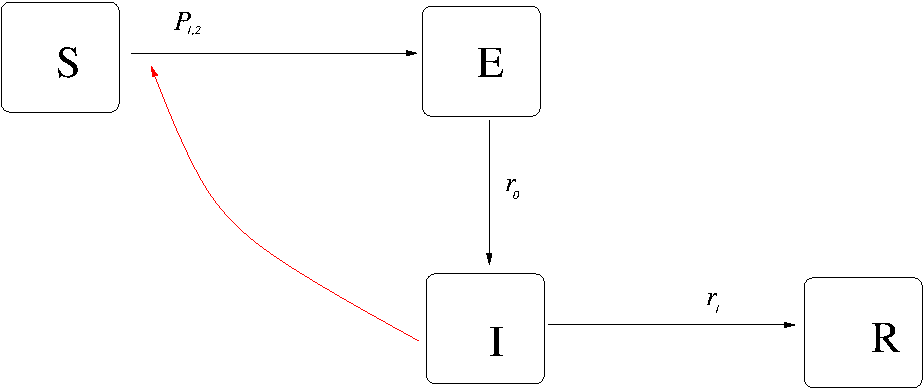
\includegraphics[scale=0.4]{images/swseir.png}
 \caption{State transition diagram} \label{fig 5.2}
 \end{figure}
 
 
 
Figure  \ref{fig 5.1}  shows the arrangement of nodes in a small world network and  figure \ref{fig 5.2} show the transmission state diagram: S to E based on the small world network network structure and the infection probabilities $p_{1,2}$: E to I with probability $r_0$ and I to R with probability $r_1$. in figure \ref{fig 5.1}, the infected green node may infect its four red near neighbours with probability $p_1$ and its three remote neighbours with probability $p_2$. By infection we mean transition from Susceptible to exposed state.

Let $p_1$ be the probability of an infected individual causing their susceptible near neighbours to become infected and $p_2$ the probability of their distant or remote neighbours to be come infected. Exposed people become infectious with probability $r_0$ and recover or get removed with probability $r_1$. In addition $n_1$ and $n_2$ is number of close neighbours and near neighbours respectively.

The number of distant neighbours $n_2$ if fixed and random for each node. That is for node i there are $n_2^{(i)} $ distant neighbours. $n_2^{(i)} $ is chosen to follow a discrete exponentially decaying distribution 
\begin{equation}
f_c(x) = \dfrac{1}{c} e^{\dfrac{-x}{\mu}}
\end{equation}
with  parameter $\mu$ proportional to the expected number of links to remote nodes and $c = \frac{1}{1- e^{frac{-1}{\mu}}}$ ensures that $f_c$ is a probability distribution function \citep{fu2013propagation}. The degree distribution in most social networks are exponentially distributed because of the celebrity effect \citep{estrada2015first}. In social networks there are few people who are with high connections and many with an average number of connections. In modelling infectious diseases these individuals are referred to as supper spreaders.

The transition probability $r_0$, the number of days an individuals is in the exposed state is as a result of bernoulli trials with mean $\frac{1}{r_0}$, follows a geometric distribution $f_X(x) = (1-p)^{x-1}p$. Similarly the infectious period follows a geometric distribution with mean $\dfrac{1}{r_o}$ \citep{fu2013propagation}.

\section{Model}
The model has seven parameters, the are $N, p_1,p_2, n_1, n_2,r_0$ and $r_1$. We let $N$ be the population size of a city or  country and is arranged in a regular grid  of side length $l $ such that $l^2 = N$. The rest of the parameters have been described above.

A  thorough review of literature in \cite{lessler2016times} indicates that $95 \%$ of patients begin to exhibit symptoms of Zika infection after $11.2$ days of infection with a $95 \%$ confidence interval of $7.6 -18$. Further the center for disease control and prevention (CDC) indicate that the incubation period for Zika virus ranges for 3 day to 14 days from infection \citep{krow2017estimated}. Therefore we estimate $r_o$  with $\frac{1}{11.2}$

$95\%$ of the cases will still have detectable virus infectiousness 18.9 days after infection with a confidence interval of 13.6 -79.4  \citep{lessler2016times}.The infectiousness in Zika infection ends 1.5 - 2 days before the virus becomes undetectable \citep{funk2016comparative}. Thus the chosen value for infectious period id $18.9 - 1.5 = 17.4$ days. Therefore $r_1$ is estimated  to be $\frac{1}{17.4}$.

Hence we have $n_1$, $\mu$, $p_1$ and $p_2$ free parameters. Without control the average number of secondary infection for Zika virus is between 3 and 6, therefore we choose 4.5 as the $R_0$. Since the number of remote neighbours is random and fixed for each, we estimate $E (n^{(i)}_2) = \mu$.

\begin{align}
n_1 p_1 + \mu p_2 \approx \dfrac{R_0}{r_1} 
\\ n_1 p_1 + \mu p_2 \approx 0.2586
\end{align}
thus, 
$p_1 =  1.034 - 0.25 \mu p_2$

We can summarize the parameters of the models as;
\begin{align}
n_1 &= 4 \\
\mu &= 8 \\
r_0 &= \dfrac{1}{11.2} \approx 0.089 \\
r_1 &= \dfrac{1}{17.4} \approx 0.057 \\
p_1 &= 1.034 - 2 p_2
\end{align}
Now we have one free parameter. We can now estimate the number of new infections by;
\begin{align}
E(- \bigtriangleup S) = (n_1 k p_1 + \mu p_2 - r_1) I \label{5.18}
\end{align}
Where k is the average number of near neighbours' links that support possible infection and near neighbours are arrange in clusters, therefore $0.5 <k <1$. In all our computation we will take $k = 0.5$. From equation \ref{5.18} we can estimate the number of new infections as;
\begin{align}
E(- \bigtriangleup S) = (2 p_1 + 8 p_2 - 0.057) I  \label{5.1.9}
\end{align}